\chapter{Background}
\label{ch:background}

The aim of this chapter is to give the reader background information on certain areas of machine learning and
game theory in order for them to understand the rest of the report.
There will also be a in-depth discussion of existing literature that relates to machine learning in texas hold'em
agents.

Machine learning is an area of computer science that tackles how we construct computer programs that improve
with experience\citep{mitchell1997machine}.
The term was coined by Arthur Samuel in a paper in which he discussed machine learning methods using
checkers\citep{samuel1959some}.
Since then there has been a great deal of advancement in the field.
Some of the notable early contributions being the discovery of recurrent neural networks in 1982,
the advancement of reinforcement learning by the introduction of Q-Learning in 1989 and the
development of a backgammon-playing agent using neural networks and temporal difference learning\citep{tesauro1995td}.
Recently we have seen some of this early academic work culminate in more practical achievements such as
Facebook's DeepFace system which, in 2014,  was shown to be able to recognise faces at a rate of 97.35\% accuracy,
a rate that is comparable to that of humans.
Another example of recent achievement is Google's AlphaGo program which, in 2016, became the first program to beat
a professional human player.

It should be becoming clear that machine learning can be a solution to a wide array of problems and as
both hardware and software continue to improve it's reach will only continue to grow.
We are starting to see machine learning systems become a key component of many companies business model.
Since certain machine learning techniques are great at prediction, machine learning has been widely used
for content discovery by companies such as Google and Pinterest.
Other business applications include the use of chatbots as a part of customer service, self-driving cars
and even in the field of medical diagnostics.


\section{Reinforcement Learning}\label{sec:reinforcementLearning}
The early research for this project yielded reinforcement learning as the most suitable machine learning
paradigm for the problem of texas hold'em.
However, in order to understand both reinforcement learning and how it would apply to the chosen problem,
in depth research was required.
This research included a Udemy course\citep{udemy2018rlpython} as well as reading in part the book
Reinforcement Learning: An Introduction\citep{sutton1998reinforcement}.

\begin{figure}[ht]
    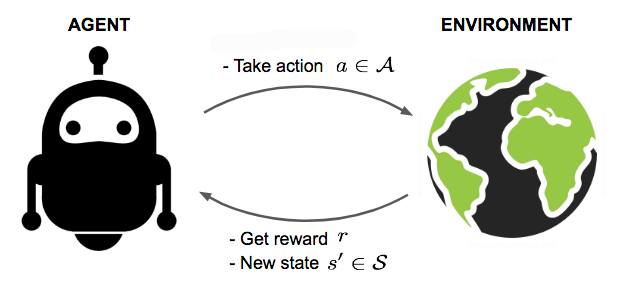
\includegraphics[scale=.5]{images/RL_illustration.png}
    \caption{Reinforcement Learning - adapted from\citep{weng2018longpeek}}
\end{figure}

As mentioned in the introduction, reinforcement learning is a method of programming agents by reward and
punishment without needing to specify how the task is to be achieved.
As such the primary components of a reinforcement learning problem are an agent which exists in an environment.
From a simplified perspective we can think of the environment as a set of states, actions and rewards.
The interaction of the agent and the environment using these three components is shown in figure 2.1.
The objective for the agent is to maximise cumulative reward.
This is done by developing a policy that will dictate which actions should be taken in each state.

\subsection{Explore-Exploit Dilemma}\label{subsec:exploreExploit}
When it comes to reinforcement learning one of the first questions that should be asked is
how the state space be explored.
An example that is often used to conceptualize this problem is the multi-armed bandit problem.
Let's say an agent is in a room with a number of gambling machines.
Each of these machines has an arm that, when pulled will return a reward of 0 or 1 based on some underlying
probability\citep{kaelbling1996reinforcement} (see figure 2.2).
The agent has a limited number of total pulls.
So the question becomes how should these pulls be distributed in order to maximise return?
Well, first, enough exploration must be performed such that the machine with the best reward probability is found
and second, this machine must be maximally exploited.

\begin{figure}[ht]
    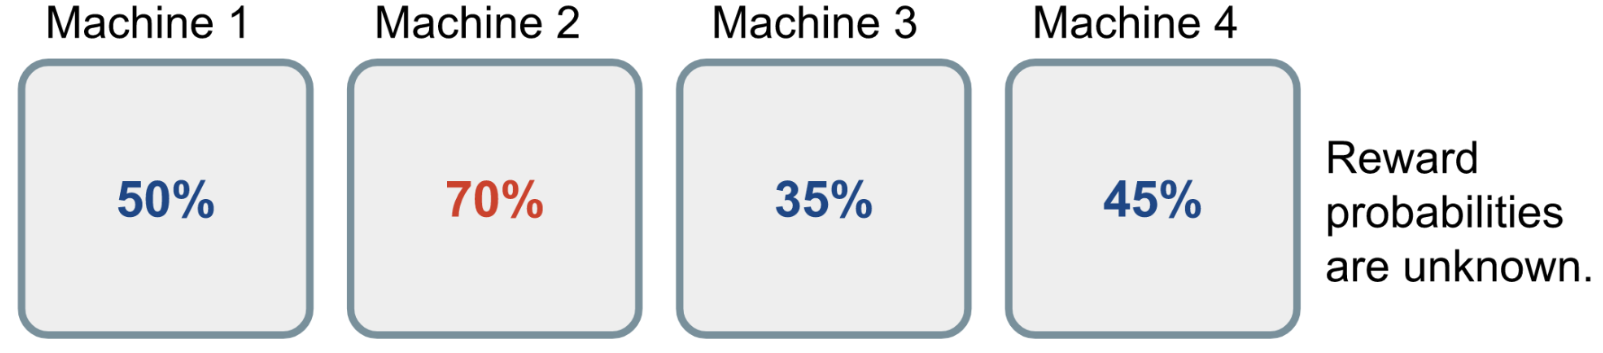
\includegraphics[scale=.25]{images/bandit.png}
    \caption{Multi Armed Bandit - adapted from\citep{weng2018multiarm}}
\end{figure}

There are a number of approaches that can be taken to solve this problem, two of these
methods will now be briefly discussed.

\subsubsection{$\epsilon$-Greedy Solutions}\label{subsec:eGreedy}
The first approach is the $\epsilon$-greedy strategy.
This approach was first proposed in\citep{watkins1989learning} and is a very simple and widely used method.
The $\epsilon$-greedy strategy involves choosing a random lever some proportion $\epsilon$ of the time, and
choosing the lever that has been established to give the highest reward the rest of the time.

There are a number of variations of this method, the first being the $\epsilon$-first strategy.
With this strategy all random choices are taken first, thus evaluating the best bandit,
after which this bandit is exploited.
However, as stated in\citep{vermorel2005multi} this simple approach is sub-optimal because asymptotically,
the constant factor prevents the strategy from getting arbitrarily close to
the optimal lever.

This is where the $\epsilon$-decreasing strategy becomes useful.
Here, the proportion of random lever pulls decreases with time.
Generally, if the initial epsilon value is $\epsilon_0$ then the epsilon value at time $t$ will be
$\epsilon_t = \frac{\epsilon_0}{t}$.

\subsubsection{Upper Confidence Bounds}
Another approach that can be used is called the upper confidence bound(UCB) method.
With this method an initial optimistic estimate of the reward of each bandit is assigned.
After which a greedy approach is taken.
Less explored bandits will have a artificially higher reward estimate and thus they will be greedily chosen,
thus allowing us to evaluate each of the bandits.

In the context of reinforcement learning, state space exploration through the $\epsilon$-greedy approach is
generally sufficient.

\subsection{Markov Decision Processes}\label{subsec:mdp}
In the last section some methods that can be used to explore environments have been established.
The next step is to discuss in more detail how reinforcement learning environments, and their interaction
with reinforcement learning agents, are modelled.
Generally finite Markov decision processes (finite MDPs) are used.
Markov decision processes provide a formal mathematical framework for sequential decision making,
where actions influence immediate rewards as well as subsequent situations\citep{sutton1998reinforcement}.
MDPs allow us to create an idealized model of reinforcement learning problems and thus precise
theoretical statements can be made.

\subsubsection{MDP Dynamics}

As mentioned earlier, reinforcement learning problems consist of an agent and an environment interacting.
Markov decision processes can be looked at in a similar way.
However, there are a number of additional factors that must be considered in order to paint a complete picture.

The problem can be thought of as consisting of a set of discrete time steps.
At each time step the environment supplies the agent some information about the state, $S_t$.
Using this information the agent chooses an action, $A_t$.
Then, as a result of the action, the environment will supply the agent with a reward, $R_t$, as well as a new state.
As such the process of interaction between the agent and the environment can be seen as a trajectory of states,
actions and rewards\citep{sutton1998reinforcement}:
\begin{align}
    S_0,A_0,R_1,S_1,A_1,R_2,S_2\dots
\end{align}

Thus far it has been stated that states, actions and rewards are related, however questions still exist as to
the exact workings of this relationship.
The answer is that finite MDPs contain a discrete probability distribution that determines the likelihood that we
will reach the state $s'$ and receive reward $r$ at time $t$ based on the previous action $a$ and state $s$:
\begin{align}
    p(s',r|s,a) \doteq \Pr\{S_t=s',R_t=r|S_{t-1}=s,A_{t-1}=a\}
\end{align}
In simplified terms this means that for a given state-action pair $(s,a)$, the probability of us reaching some
new state $s'$ and receiving reward $r$ is determined by the MDPs probability function $\Pr$.

This four argument probability function completely characterizes the dynamics of the MDP and from it any other
information about the environment can be obtained\citep{sutton1998reinforcement}.

\subsubsection{MDPs and Learning}
The goal of the agent in an MDP is to learn how to maximise the cumulative reward received when traversing
the environment.
In some cases the MDP will be traversed until a terminal state, $T$, is reached.
This type of MDP reflects episodic tasks that will always terminate.
In this case cumulative reward,$G_t$ can be calculated as follows:
\begin{align}
    G_t = R_{t+1}+R_{t+2}+R_{t+3}+\dots+R_T
\end{align}

However, in other cases continuous tasks are modelled.
The problem here is that, if the same method of calculating $G_t$ is used then in this case $G_t$
will always eventually sum to infinity, regardless of whether good or bad actions are being selected.
As such a concept called discounting must be introduced.
With this approach the aim is to maximise the sum of future discounted rewards.
Thus $\gamma$, a parameter with a value between 0 and 1, is utilised.
As such, for continuous tasks modelled as MDPs our cumulative reward is as follows:
\begin{align}
    G_t = R_{t+1}+\gamma R_{t+2}+\gamma^{2}R_{t+3}+\dots
\end{align}

Based on our specified value of $\gamma$ the weighting of future rewards can be adjusted.
For example if a low value for $\gamma$ (eg .5) is used then the value of rewards more than a
few time steps in the future will be very low.

\subsubsection{Partially Observable Markov Decision Processes}
A partially observable Markov decision Process (POMDP) is used to model environments that are not
fully observable\citep{kaelbling1996reinforcement}.
POMDPs extend MDPs by including a set of observations, $O$.
There is also an observation function, $P(O_t=o|S_t=s)$, that determines the probability of making a certain observation
in a certain state.
Hold'em can be modelled as a POMDP due to the fact that is an imperfect information game.

However, it is possible that an agent in a POMDP environment can remember the sequence of observations
and actions that lead to the current state.
This is a sufficient statistic of it's experience and can thus define a complete information
state\citep{heinrich2017reinforcement}.
As such a POMDP can be reduced to it's underlying MDP by using these full history information
states and also extending the relevant transition and reward functions.


\subsection{Policy Evaluation and Policy Improvement}\label{subsec:policyEvalPolicyImp}
As mentioned above the primary focus of reinforcement learning is to find a policy (denoted by $\pi$) that allows
the agent to take actions in states that lead to the maximum possible reward.
There are two primary problems that must be solved in order to do so.

The first is called the prediction problem, or policy evaluation.
This involves computing the values of states given some arbitrary policy\citep{sutton1998reinforcement}.
For example a state would have a high value if the reward for reaching that state was high.
A state would also have a high value if the current state was only one action away,
according to the supplied policy, from a state that renders a high reward.
However a state would have a low value if, according to the policy, there was no path to a state that
would return a positive reward in the foreseeable future.

The second problem is known as the control problem, or policy improvement.
This involves changing the policy in order to improve our cumulative reward.
The policy improvement process can only occur when policy evaluation has been performed.
Let's say, after our evaluation step, the value of some state $s$ is known.
Note that this value is calculated with the condition that some action $a$ is taken in state $s$.
But, if some other action $a'$ is taken, would this render a higher value for $s$?
If the answer is yes then the policy is updated.

These two operations can be seen as the core of reinforcement learning.
In the next section different reinforcement learning methodologies will be discussed.
Some of the main differences are in how method each approaches the prediction and control problems.

\subsection{Dynamic Programming}\label{subsec:dp}
Dynamic programming (DP) refers to a collection of algorithms that can be used to compute optimal policies given a
perfect model of the environment as a Markov decision process\citep{sutton1998reinforcement}.
DP is not widely used in practical reinforcement learning applications due to its assumption
of a perfect MDP and it's high computational requirements.
Despite this it is very important from a theoretical standpoint as it serves as an introduction to a number
of important reinforcement learning concepts.
Furthermore, it provides a basis for many algorithms that are used in practical reinforcement learning applications.

\subsubsection{Policy Evaluation in Dynamic Programming}
When discussing policy evaluation a state-value function or a value function is referred to.
This is simply the mapping of states to their corresponding values and is denoted by $v$.

Since the environments's dynamics are completely known, an iterative solution to finding
the value function can be applied.
If a series of approximate value functions $v_0, v_1, v_2,..$ are considered.
The initial value function, $v_0$ is chosen arbitrarily and each successive generation is obtained by
using the Bellman equation for $v_\pi$ as an update rule\citep{sutton1998reinforcement}:

\begin{align}
    v_{k+1}(s) &= \EX_{\pi}\lbrack R_{t+1} + \gamma v_k(S_{t+1}) | S_t = s \rbrack
\end{align}

In order to produce each successive approximation of $v_{k+1}$ from $v_k$ the operation outlined to each
state $s$ is applied.
As shown above the new value for $s$ is based on a combination of the expected immediate rewards($R_{t+1}$),
and the expected values of each of the states that can be transitioned to($S_{t+1}$) given policy $\pi$.
It can be shown that as $k\rightarrow\infty$ $v_k$ will converge to $v_\pi$, the correct value function for policy
$\pi$.
This algorithm is called \textit{iterative policy evaluation}\citep{sutton1998reinforcement}.

\subsubsection{Policy Improvement in Dynamic Programming}
Since the value of following $v_\pi$ is known, this information can be used to determine how
this policy should be modified in order to improve its value.
Assume that $\pi$ is a deterministic policy.
This means that $\pi(s)$ will return some action that must be taken.
Now the question becomes what if some other action $a \neq \pi(s)$ is taken?
This depends on whether or not choosing this action, and then continuing to use the existing policy will
improve the value of the policy.
If it does then this new action will be chosen.

The logical extension of this approach is to apply it to each state and each possible action.
As a result, what appears to be the best action at each state will be selected.
The new greedy policy $\pi'$ can be denoted as:
\begin{align}
    \pi'(s) = argmax\EX_{\pi}\lbrack R_{t+1} + \gamma v_k(S_{t+1}) | S_t = s, A_t = a\rbrack
\end{align}
Essentially here the value of each available action in the current state is determined using the same operation
as outlined in the policy evaluation phase.
Then the argmax function will select the action with the highest value.
Finally, this action is assigned to be the one that will be choosen in state s, according to the new policy $\pi'$.

Note that in this section an algorithm has been outlined with respect to deterministic policies,
however a lot of times in reinforcement learning deals with stochastic policies.
This means that actions are taken in states according to some probability distribution rather than always choosing
the same action in a particular state.
This is not a problem as the ideas mentioned apply equally well to stochastic policies.

\subsection{Monte Carlo}\label{subsec:mc}
Monte Carlo(MC) methods are a wide range of algorithms that rely on random sampling in order to obtain results.
Such a method could be applied in the case of having an array of 1 trillion elements that could be
either 1 or 0.
In order to calculate the number of 1s in such an array iteration could be used.
However, this would be extremely computationally costly.
Instead, random indices could be generated to sample the array.
A count of both the number of 1s found and the number of indices generated would be maintained.
Based on these figures it would be possible to estimate the total number of 1s in the array.
Over time as more samples are taken the estimate would converge towards the true value.

Monte Carlo based reinforcement learning techniques apply this method in the policy evaluation step.
In Monte Carlo, unlike dynamic programming, there is no assumption of complete knowledge of the environment.
Monte Carlo methods require only experience.
Sequences of states, actions, and rewards are sampled from interaction with the
environment\citep{sutton1998reinforcement}.
These sequences are called episodes.
Monte carlo evaluation is an episodic process.
This means that action values are only updated after an episode has completed.

\subsubsection{Monte Carlo Policy Evaluation}
In Monte Carlo methods a fundamentally different approach to policy evaluation is taken.
As mentioned this method is focused on using episodic experience.
In order to evaluate a state the rewards returned after visiting that state are averaged.
As more returns are observed the average will converge to the actual expected value of the state.

It is worth noting that a state $s$ could be visited more than once in an episode.
As such, the returns can either be averaged following the first visit to $s$ or averaged
after each visit to $s$.
These two methods are called \textit{first-visit} and \textit{every-visit} respectively.

\subsubsection{Monte Carlo Action Values}
In Monte Carlo methods, the lack of a model means that state values are insufficient in order to
obtain a policy.
Rather state-action pairs are generally evaluated.
This mapping of state-action pairs to values is referred to as the $q$ function or the action value function.
In this case the evaluation problem for action values is to estimate $q_\pi(s, a)$, the expected return when
starting in state s, taking action a, and thereafter following policy $\pi$\citep{sutton1998reinforcement}.

The method for policy evaluation using state-action pairs is almost identical to that outlined above.
The only difference being that instead of averaging rewards for each state,
rewards for each action taken when a state is visited are averaged.
There is one problem with this approach in the context of deterministic policies.
The problem being that in following a deterministic policy rewards will only be returned
for a single action, thus only one action value estimate will be improved.
In order to negate this problem it can be specified that every episode begin in a state-action pair,
with the probability of starting in each state-action pair being non-zero.
This is called the \textit{exploring-starts} method.
Another approach would be to ensure that a stochastic policy is used with
the probability of selecting each action being non-zero.

\subsubsection{Monte Carlo Policy Improvement}
In Monte Carlo methods, the overall policy improvement algorithm is the same as outlined in the dynamic
programming section.
That is, it alternates between modifying the value function to more closely approximate the current policy,
and using the value function to improve the policy.
However, as mentioned, in the case of Monte Carlo a $Q$ function is used as shown in figure 2.3.
\begin{figure}[ht]
    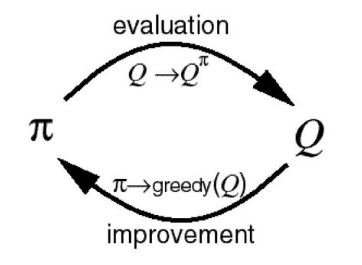
\includegraphics[scale=.5]{images/MC_control.png}
    \caption{Monte Carlo Policy Improvement - adapted from\citep{lee2005mccontrol}}
\end{figure}

\subsection{Temporal Difference Learning}\label{subsec:td}
The final reinforcement learning method that will be discussed is the Temporal Difference(TD) learning method.
TD learning combines dynamic programming(DP) and and Monte Carlo(MC) ideas\citep{sutton1998reinforcement}.
Like MC, learing occurs directly from experience, without a model of the environment's dynamics.
However, like DP state value estimates are updated based on other learned estimates, without needing to wait for an
episode to complete and the return of some final outcome.

The selective use of different aspects of these reinforcement learning methodologies by TD learning has
a number of advantages.
The fact that a model of the environment is not needed makes it easier to implement TD methods
compared to DP .
TD methods are also conducive to solving problems with long episodes or even continuous tasks with no
episodes at all due to the fully online nature of this learning algorithm.

\subsubsection{TD Learning Policy Evaluation}
Unlike MC, with TD learning the value function can be updated at every time step.
This is exemplified by the \textit{TD(0)} or \textit{one-step TD} method in which the
update is made immediately on transition from state $S_t$ to state $S_{t+1}$.
The more general case of this method is the \textit{TD($\lambda$)} or \textit{n-step TD}.
With \textit{TD(0)} the update rule is as follows:
\begin{align}
    V(S_t) \leftarrow V(S_t) + \alpha \lbrack R_{t+1} + \gamma V(S_{t+1}) - V(S_t) \rbrack.
\end{align}
As such the new value for some state $S_t$ is dependant on the previous value of the state($V(S_t)$),
along with the reward($R_{t+1}$) gained from transitioning to state $S_{t+1}$ plus the discounted($\gamma$)
estimated value of that state($V(S_{t+1})$).
The sum of the latter is multiplied by $\alpha$ which is a small positive fraction that influences the
learning rate.

This rule is applied for each state visited in an episode and for each episode.

\subsubsection{TD Learning Policy Improvement - SARSA}
At this point it is worth noting that there are two distinct methods of handling policy improvement.
The first is on-policy and the second is off-policy.
On-policy reinforcement learning is when the policy being evaluated or improved is the same policy that is used
to make decisions.
In off-policy reinforcement learning the policy being used to generate behavior is not the same as the policy
being evaluated or improved.

SARSA is an example of an on-policy algorithm.
The policy improvement mechanism is the same here as outlined in the previous sections.
With SARSA, like in Monte Carlo the action-value function($q_{\pi}(s, a)$) is utilised rather
than the state-value function.
Thus the policy evaluation step is slightly modified as follows:
\begin{align}
    Q(S_t, A_t) \leftarrow Q(S_t, A_t) + \alpha \lbrack R_{t+1} + \gamma Q(S_{t+1}, A_{t+1}) - Q(S_t, A_t) \rbrack.
\end{align}
This update utilises the quintuple of events, ($S_t, A_t, R_{t+1}, S_{t+1}, A_{t+1}$), which is where the
name SARSA originates.


\subsubsection{TD Learning Policy Improvement - Q-Learning}
Q-Learning is an off-policy control algorithm.
This was one of the early breakthroughs in reinforcement learning as it allows the direct approximation of
the optimal action value function independent of the policy being followed.
The update rule is as follows:
\begin{align}
    Q(S_t, A_t) \leftarrow Q(S_t, A_t) + \alpha \lbrack R_{t+1} + \gamma maxQ(S_{t+1}, a) - Q(S_t, A_t) \rbrack.
\end{align}
Here our update rule is similar to that of SARSA apart from the fact that the value of the best
action available ($maxQ(S_{t+1}, a)$) is used when updating our action value.

\subsection{Monte Carlo Tree Search}\label{subsec:mcts}
In this section Monte Carlo Tree Search(MCTS), a decision time planning algorithm will be discussed.
This iterative algorithm uses tree search combined with value estimations from MC simulations in order to
efficiently solve very large MDPs.
One application of this algorithm was in DeepMind's AlphaGo\citep{silver2016mastering} which became the
first computer program to beat a highly ranked Go champion.

\begin{figure}[!ht]
    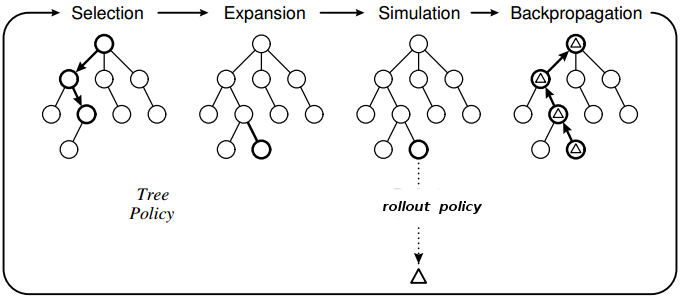
\includegraphics[scale=.8]{images/MCTS.png}
    \caption{MCTS - adapted from\citep{lim2016field}}
\end{figure}

MCTS is an episodic process.
As shown in figure 2.4, there are four key steps involved in each of these episodes.
The first step is \textbf{selection}.
From the root of the tree, the tree policy is used.
This policy is based on action values associated with the edges of the tree, in order
to select a child node at each level\citep{sutton1998reinforcement}.
The second step is \textbf{expansion}.
When a leaf node is reached in the tree, one or more child nodes may be added based on
the actions available at that point.
The third step is \textbf{simulation}.
When the tree has been exited the rollout policy is used in
order to provide default behavior outside of the tree and ultimately reach a
terminal node from which a reward can be obtained.
The final step is \textbf{backpropagation}.
This step is uses the reward obtained to update the values of the tree nodes that were visited
during the episode.

In summary this algorithm uses the simulation step in order to efficiently sample rewards which
are then propagated back to nodes of the tree.
In later iterations the tree policy selects which areas of the tree to
explore based on these propagated values.
In section 2.4 a method for applying MCTS to imperfect information games such as poker will be outlined.

\section{Game Theory}\label{sec:gameTheory}
After taking a deep dive on reinforcement learning and the papers surrounding RL in texas hold'em it became
clear that a pure reinforcement learning approach would not be feasible.
The main reason for this was the fact that texas hold'em is an imperfect information game.
As outlined by\citep{dahl2001reinforcement}:
\begin{quotation}
Note that the concept of game state values, which is the key to solving perfect information games,
does not apply to imperfect information games, because the players do not know from  which game states they
are choosing.
\end{quotation}
As such it became apparent that some other techniques would have to be incorporated in order to create a competent
texas hold'em agent.
After discovering the following two key papers\citep{heinrich2016deep} and\citep{heinrich2017reinforcement},
the initial goal was to utilise the Neural Fictitious Self-Play(NFSP) method as a basis for our agent.
Eventually, instead it was decided that MCTS would be used as the basis for our agent implementation.
NFSP is based heavily on the game theoretic concepts that are outlined in this section, however,
the MCTS implementation that is discussed later will rely on a number of these concepts.

\subsection{Modelling Games}\label{subsec:modellingGames}
When an attempt is made to solve a game, the way in which the game is modelled must first be understood.
It is also important to carefully consider how a form or structure of the model is defined\citep{myerson2013game}.
In this section three important forms that games can take will be discussed.
The varying utility of each of the different scenarios will also be outlined.

\subsubsection{Extensive Form Games}
Extensive form games are a model of players sequential interaction, with explicit representation of a
number of key aspects of the game.
\citep{kuhn2016extensive} formally defined extensive form games as consisting of the following components:
\begin{itemize}
    \item \textit{N} - a set of players.
    \item \textit{S} - a set of states that represent the nodes of a rooted game tree.
    \item \textit{A(s)} - a set of actions for each state representing the edges to the following states.
    \item \textit{U} - a set of information states (one set for each player).
    \item \textit{Player Function} - determines who is to act at a given state.
    \item \textit{Information Function} - determines which states are indistinguishable for the player by mapping them to the same information state.
    \item \textit{Return Function} - maps terminal states to each player's return/payoff.
\end{itemize}

Extensive form games allow us to richly describe game situations.
This allows us to uncover characteristic differences between games and the structural features which
determine these differences\citep{kuhn2016extensive}.

Behavioral strategies for players can also be defined.
These consist of a probability distribution over actions
given information states\citep{heinrich2017reinforcement}.
This is denoted by $\pi^i(a|u^i)$.
If there exists a collection of strategies for all players in the game then this is called a strategy profile, $\pi$.
$\pi^{-i}$ is the set of strategies in $\pi$ not including $\pi^i$.
This will be discussed later when Heinrich's implementation is discussed in more depth.

\subsubsection{Normal Form Games}
Normal form games are represented by way of a matrix.
Although some information is lost in comparison to extensive form games, normal forms are
better suited to the derivation of generalized theorems\citep{kuhn2016extensive} and thus have their own utility.

An extensive-form game can induce an equivalent normal form of the same game.
This can be done through the generation of a set of deterministic behavioral strategies for each player
called pure strategies.
Each pure strategy is a full game plan that will determine an action for each situation the player may encounter.
Mixed strategies can also be created which define a probability distribution over the players pure strategies.
A mixed strategy for player $i$ is denoted as $\Pi^i$.
When the extensive-form return function is restricted to normal-form the yield is an expected return function.
The expected return function for some mixed strategy profile $\Pi$ is $R^i(\Pi)$\citep{heinrich2017reinforcement}.

\subsubsection{Sequence Form Games}
In order to compute a Nash equilibrium for an extensive form game the game can be converted to a normal form,
however normal forms tend to produce very large game trees.
The sequence form is an efficient method of representing extensive form games\citep{koller1996efficient}.
This representation is described as a linear-sized strategic description of the game.
It decomposes players strategies into sequences of actions and probabilities of realizing those sequences.

In sequence form games, for every player $i\in N$, each of their information states $u^i\in U^i$
uniquely define a \textbf{sequence} $\sigma_{u^i}$ of actions that a player must take in order to reach
that information state.
These sequences are then mapped to realization probabilities through what is called a realization plan,
denoted by $x$.
When two or more strategies have the same realization plan these strategies are considered to be
realization equivalent\citep{von1996efficient}.
This can apply across different types of strategies for example extensive-form, behavioral strategies
and normal-form, mixed strategies\citep{kuhn2016extensive}.

\subsection{Nash Equilibria}\label{subsec:nashEquilibria}
A Nash's equilibrium is a state in which each player in a game has chosen a strategy and
none of the players can benefit from changing their strategies, if the other player's strategies remain unchanged.
As such, if a strategy is developed that induces a Nash's equilibrium our strategy can no longer be exploited.

In the context of extensive form games the concept of best responses is related to that of Nash's equilibria.
If the opponent's strategies are denoted by $\pi^{-i}$ then the set of best responses are denoted by
$BR^i(\pi^{-i})$.
Note that for a strategy profile $\pi$ such that $\pi^i\in BR^i(\pi^{-i})$ for every $i\in N$ (i.e
for every player) then that game constitutes a Nash equilibrium\citep{heinrich2017reinforcement}.
Heinrich also discusses the concept of $\varepsilon$-best responses.
This is the set of strategies that are within a certain tolerance $\varepsilon$ of the best responses.
As such an $\varepsilon$-Nash equilibrium can be defined as a strategy profile $\pi$ such that
$\pi^i \in BR^i_\varepsilon (\pi^{-i})$ for all $i\in N$.

\subsection{Fictitious Play}\label{subsec:fictitiousPlay}
Fictitious play(FP) is a game-theoretic model of learning through self-play.
At each iteration players choose the best responses to their opponents average
strategies\citep{heinrich2017reinforcement}.
These strategies converge to Nash equilibria in certain classes of games, including two-player, zero sum games.

Generalised weakened fictitious self-play (GWFSP) is a method that is built on FP but allows for approximations
in players strategies\citep{leslie2006generalised}.
Thus it is more suitable for machine learning.
GWFSP allows for a certain error at each iteration of the algorithm and relies on the fact that this
error rate will tend towards zero as time progresses.
In the the research done by Leslie and Collins normal form games were studied.
There has also been research done into the applicability of FP to extensive form games however,
before\citep{heinrich2016deep} there was no method shown to converge for imperfect information games such as poker.
In later sections we will discuss how Heinrich utilised GWFSP as a basis for neural fictitious self-ply,
a method that has shown success in games of imperfect information.

\section{Texas Hold'em}\label{sec:thIntro}
Although it was decided that a full scale implementation for Texas hold'em would be beyond the
scope of this project, this was the target game at the inception of the project.
As such the mechanics of this game will now be discussed.
The reader may choose to skip to section 2.3.4 in order to only learn about the game of Leduc Hold'em.

Texas hold'em is one variant in a family of games called poker.
Poker is a group of card games that combine gambling, strategy and skill.
All poker variants have three core similarities.
There is betting involved, there is imperfect information (ie cards remain hidden until the end of a hand)
and the winner is determined by combinations of cards.

\subsection{Game Structure}\label{subsec:bettingRounds}
Texas hold'em consists of four betting rounds.
Initially each player is dealt two private cards.
These remain face down and only the person who received these cards may view them.
In the next three rounds five public cards are dealt face up on the table.
The second round of dealing is called the flop, where three public cards are dealt.
The third round is called the turn where one additional public card is dealt.
Finally in the fourth round another public card is dealt which is called the river.

At each round, after the cards are dealt, the players are given the opportunity to take a number of betting
related actions.
The next section outlines the permitted actions.

In order for players to be incentivized to continue playing in a wider array of situations, blinds are required.
Blinds are a mandatory bet that must be posted by two of the players present at the game.
These two bets are called the big blind and the small blind, the big blind being twice that of the small blind.
As hands are played the big and small blinds are posted by different players in order to distribute the cost fairly.

The big and small blind are the first two bets that contribute to what's called the pot.
The pot is the collection of all of the current chips bet by the players.
When a player wins a hand then what they receive in return is the pot.

The final structural component of the game is player stacks.
Each player will start the game with a certain amount of chips.
If a player wins a pot then all of the chips in the pot are transferred to the winners stack.

\subsection{Actions}\label{subsec:actions}
As mentioned in the previous section, after cards are dealt players are permitted to take a number of actions.
If a player is the first to act the they may either check or bet a chosen amount.
If a player is not first to act and the previous player has made a bet then they may choose
to either fold and forfeit the pot, call the bet by adding the same amount to the pot, or raise by
adding the amount previously bet plus some additional chips.
Players can go back and forth with bets until they run out of chips in which case they are
considered to be "all in".

\subsection{Hand Values}\label{subsec:handValues}
In poker the best 5 cards available to the player can be played.
This means any combination of his own private cards and the public cards can be used.
There are 10 major poker hands.
These are listed below in ascending order of value:
\begin{enumerate}
    \item \textbf{High Card:} None of the higher hand values achieved, highest card plays.
    \item \textbf{Pair:} Any two cards of the same rank.
    \item \textbf{Two Pair:} Two different pairs.
    \item \textbf{Three of a kind:} Three cards of the same rank.
    \item \textbf{Straight:} Five cards in a sequence.
    \item \textbf{Flush:} Five cards of the same suit.
    \item \textbf{Full House:} Three of a kind with a pair.
    \item \textbf{Straight Flush:} Five cards in sequence, all of the same suit.
    \item \textbf{Royal Flush:} A, K, Q, J, 10 - all of the same suit.
\end{enumerate}

\subsection{Leduc Hold'em}\label{subsec:leducHoldem}
Leduc Hold'em is a simplified version of Hold'em that was first introduced in\citep{southey2012bayes}.
In Leduc Hold'em the deck is reduced to six cards with two suits and three ranks in each suit.
Rather than four rounds there are only two.
In the first round a single private card is dealt to each player.
In the second round a single board card is revealed.
In the first round both players have a mandatory bet of one and a raise of two is allowed.
In the second round players can raise by four.
Each round allows for at most two bets.


\section{Variations of MCTS Applied to Poker}\label{sec:mctsPoker}
As mentioned in section 2.1.7 MCTS has been shown to be a very powerful method for solving large
perfect-information games such as Go.
However if this algorithm is to be applied to a imperfect information game like poker then
a number of modifications must be applied.
Such an approach was outlined in\citep{heinrich2017reinforcement} in which a variation of
MCTS called smooth UCT was implemented to tackle both leduc hold'em and limit hold'em.

\subsection{Extensive Form MCTS}\label{subsec:extensiveMCTS}
One of the subtleties of poker is that player information is asymmetric.
In other words each player has access to their own private card 
information but not to their opponents private cards.
This means that the search tree cannot be a single, collective
entity\citep{heinrich2017reinforcement}, rather two search trees must be available 
to accommodate self-play.
The method that can be used to accomplish this goal is the creation of
an information function $I^i(s)$, a concept from game theory(see section 2.2.1).
This function will return the information state $u^i$ of the current player ($i$) given
the current state $s$ from the full game tree.
Note that the full game tree will have separate nodes for any variation
in either player's cards.
However, player 1's game tree will not have separate nodes where the only 
differentiating factor is player 2's private cards\citep{johanson2011accelerating} 
due to the fact that this information is not available.
For example let's say that state $s$ is in the full game tree and contains the information
that player 1 has an ace, player 2 has a king and there has been a single bet so far in the game.
If this state is passed to player 1's information function the returned information
state,$u^i$, will only contain the information that player 1 has an ace and there has been a single bet thus far.
Algorithm 1 shows Heinrich's extensive form MCTS .

\begin{algorithm}[H]
    \DontPrintSemicolon
    \LinesNumbered
    \SetKwFunction{FSearch}{SEARCH}
    \SetKwFunction{FRollout}{ROLLOUT}
    \SetKwFunction{FSimulate}{SIMULATE}
    \SetKwProg{Fn}{Function}{:}{}
    \Fn{\FSearch{}}{
        \While{Within computational budget}{
        SIMULATE($s_0$)\;
        }
        \KwRet $\pi_{tree}$ \;
    }
    \Fn{\FRollout{$s$}}{
        $a \sim \pi_{rollout}(s)$\;
        $s' \sim G(s,a)$\;
        \KwRet SIMULATE($s'$)\;
    }
    \Fn{\FSimulate{$s$}}{
        \If{ISTERMINAL($s$)}{
            \KwRet $r \sim R(s)$
        }
        $i = $ PLAYER($s$)\;
        \If{OUT-OF-TREE($i$)}{
            \KwRet ROLLOUT($s$)
        }
        $u^i = I^i$($s$)\;
        \eIf{$u^i \notin T^i$}{
            EXPANDTREE($T^i$,$u^i$)\;
            $a \sim \pi_{rollout}$($s$)\;
            OUT-OF-TREE($i$) $\leftarrow$ \textbf{true}
        }{
            $a$ = SELECT($u^i$)
        }
        $s' \sim G(s,a)$\;
        $r \leftarrow $ SIMULATE($s'$)\;
        UPDATE($u^i$,$a$,$r^i$)\;
        \KwRet $r$
    }
    \caption{Extensive Form Monte Carlo Tree Search}
\end{algorithm}

Aside from the differences mentioned, extensive form MCTS remains essentially the same as generic MCTS .
On lines 6 to 9 the rollout function is listed.
Here an action is sampled using the rollout policy which is then used to generate a subsequent
state through invocation of the state transition function $G$.

The SIMULATE function is the core recursive driver behind the MCTS algorithm.
Initially, we check if we have reached a terminal state, if so the reward function,
$R$, is utilised to calculate this reward which is then returned.
Next, on line 14, the PLAYER function is used to determine which player is next to move.
Then we check a data structure called OUT-OF-TREE that keeps track of which player has
left the scope of their search tree in the current episode\citep{heinrich2017reinforcement}.
If we are outside the scope of the tree then we utilise the ROLLOUT function.
Lines 19 to 22 handle the case in which the current information state, $u^i$ is
not in player $i$'s tree, $T^i$.
In this case, this node is added to the tree using the EXPANDTREE function, and we begin
to use the rollout policy to generate behavior.
On line 24 we have the contrary case in which we continue to use the tree policy by
invoking the SELECT function.
On lines 26 to 29 the next state is generated after which the SIMULATE function is recursively
called.
When this recursion ends, the UPDATE function is called in order to update the
values and visitation counts of $u^{i}$ and it's child node.


\subsection{UCT}\label{subsec:UCT}
In order to understand smooth UCT we must first explain the meaning of UCT .
The abbreviation UCT refers to upper confidence bound(UCB) applied to trees.
This means that in the action selection portion of the algorithm a UCB approach 
is taken, where less explored nodes in the tree are given a positive bias in value.
This means that unexplored nodes will be explored which ensures that
the best actions at each position in the tree are discovered.
The value of an action is denoted as follows:

\begin{align}
Q(u^i, a) + c \sqrt{\log N(u^i) / N(u^i, a)} 
\end{align}

In this expression the $Q$ function denotes the current value estimates for each action $a$ 
in information state $u^i$.
$N(u^i)$ and $N(u^i, a)$ denote the visitation count of the information state $u^i$
and the subsequent information state after action $a$ has been taken.
The visitation count of a state is simply the number of times the algorithm has passed
through that state.
Additionally, $c$ is the exploration constant.
This constant can be used to control the level of exploration during the execution of the algorithm,
with a value of 0 resulting in a purely greedy approach.
This extension of the extensive form MCTS algorithm is shown in Algorithm 2.

\begin{algorithm}[H]
    \DontPrintSemicolon
    \LinesNumbered
    \SetKwFunction{FSelect}{SElECT}
    \SetKwFunction{FUpdate}{UPDATE}
    \SetKwProg{Fn}{Function}{:}{}
    SEARCH, SIMULATE, and ROLLOUT as in Algorithm 1\;
    \Fn{\FSelect{}}{
    \KwRet $argmax_a Q(u^i,a) + c\sqrt{\dfrac{\log{N(u^i)}}{N(u^i,a)}}$ \;
    }
    \Fn{\FUpdate{$u^i$,$a$,$r^i$}}{
    $N(u^i) \leftarrow N(u^i) + 1$\;
    $N(u^i,a) \leftarrow N(u^i,a) + 1$\;
    $Q(u^i,a) \leftarrow Q(u^i,a) + \dfrac{r^i-Q(u^i,a)}{N(u^i,a)}$
    }
    \caption{UCT}
\end{algorithm}

\subsection{Smooth UCT}\label{subsec:smoothUCT}
Smooth UCT is a modification of UCT that is inspired by fictitious play\citep{heinrich2017reinforcement}.
As described in the last section the action selection in UCT is purely deterministic.
Smooth UCT changes this by utilizing the average strategy a certain proportion of the time.
In order to calculate the average strategy for a particular state we create a 
probability distribution based on the visitation counts of the actions 
available at that state.
For example, we could have an information state $u^i$ that has been visited 100 times
and has three available actions, $a_1, a_2, a_3$.
Then it would be possible that $a_1$ has been visited 50 times, $a_2$ 35 times 
and $a_3$ 15 times.
According to the average strategy we would then select $a_1$ 50\% of the time, 
$a_2$ 35\% of the time and $a_3$ 15\% of the time.
This process can be seen on line 9 and 10 of Algorithm 3.
Here, for each available action $a$ at information state $u^i$ we set the
probability of selecting that action to be the visitation count of the child node ($N(u^i,a)$)
divided by the visitation count of the parent ($N(u^i)$).
In order to determine when the average strategy should be used compared to the 
UCB approach Heinrich describes a sequence $\eta_k$.
This sequence decays to 0 as $\lim_{k \to \infty}$ and is expressed as follows:

\begin{align}
\eta_k = max(\gamma, (1 + d * \sqrt{N_k})^{-1})
\end{align}

Here $N_k$ is the total number of plays, $\gamma$ is a lower limit on $\eta_k$
and $d$ is a constant that parametrises the rate of decay.
This is calculated on line 4 of Algorithm 3.

\begin{algorithm}[H]
    \DontPrintSemicolon
    \LinesNumbered
    \SetKwFunction{FSelect}{SELECT}
    \SetKwProg{Fn}{Function}{:}{}
    SEARCH, SIMULATE and ROLLOUT as in Algorithm 1\;
    UPDATE as in Algorithm 2\;
    \Fn{\FSelect{}}{
    $\eta \leftarrow max\left(\gamma, \left(1 + d * \sqrt{N_k}\right)^{-1}\right)$\;
    $z \sim U[0,1]$\;
    \eIf{$z < \eta$}{
    \KwRet $argmax_a Q(u^i,a) + c\sqrt{\dfrac{\log{N(u^i)}}{N(u^i,a)}}$ \;
    }{
    $\forall_a \in A(u^i):p(a) \leftarrow \dfrac{N(u^i,a)}{N(u^i)}$\;
    \KwRet $a \sim p$
    }
    \KwRet $\pi_{tree}$ \;
    }
    \caption{Smooth UCT}
\end{algorithm}

In chapter 3 we will take this abstract algorithm and document how it was translated to
python code.


\section{Other Approaches}\label{sec:thImplementations}
Although it has already been stated that there will be a focus on MCTS,
it's worth discussing some other notable methods for creating poker 
agents before proceeding.
Currently the premier method for tackling full-scale texas hold'em is counterfactual 
regret minimization.
This is the method that has dominated the Annual Computer Poker Competition(ACPC) for the 
last number of years, however recently some new methods have been outlined 
which look promising and thus will be discussed as well.


\subsection{Counterfactual Regret Minimization}\label{subsec:thCFR}
Counterfactual regret minimization(CFR) is a method for finding approximate Nash
equilibria in imperfect information games and was first outlined in\citep{zinkevich2008regret}.
Regret is a measure of the difference in utility between following some strategy 
$\sigma$ compared to another strategy.
Zinkevich introduced counterfactual regret which is regret applied to a 
single information set ie a single extensive form game state.
It was found that by calculating and minimizing regret on an individual
state basis that there were performance benefits as well as an improvement 
in accuracy of the calculated approximate Nash equilibria.

One implementation of CFR is outlined in\citep{jackson2013slumbot}.
This paper outlines the implementation used for Slumbot, the 2018 ACPC champion 
in no-limit hold'em.
Jackson describes his use of CFR in order to generate a static strategy that approximates
a Nash's equilibrium.
At each iteration a strategy would be computed and when the process had ended an 
average of these strategies would be used.
Jackson also mentions using an abstraction of the game in order to reduce no-limit's 
massive state space (roughly $10^{164}$ with stack sizes of 100 big blinds)\citep{johanson2013measuring}.
This is done through techniques like grouping similar hand values into buckets and 
treating them as strategically equal or splitting the game up into it's individual rounds 
and solving the rounds separately.
These techniques allow for a dramatic reduction in state space and if handled correctly, 
should allow for a strategy that can transfer to the full version of the game successfully.


\subsection{Neural Fictitious Self-Play}\label{subsec:thNFSP}
As mentioned earlier Fictitious Play(FP) is a game theoretic model that allows learning through self-play.
This model was then extended a number of times until generalised weakened fictitious play(GWFP) was developed as a
method of self-play that was applicable to machine learning techniques.
Heinrich then utilised this method to develop Fictitious Self-Play(FSP)\cite{heinrich2015fictitious}.
This is a machine learning framework that implements fictitious play.
This method was shown to successfully generate approximate Nash's equilibria in imperfect information games
such as Leduc Hold'em.

Neural Fictitious Self-Play(NFSP) develops upon these methods through the use of neural
networks in order to facilitate the larger state spaces of games such as limit texas hold'em.
This method was outlined in\cite{heinrich2016deep}.

\subsubsection{Algorithm}
NSFP agents learn through self play ie interaction with other instances of the agent.
As this process is happening the agents store experience of their play in two memories
named $M_{RL}$ and $M_{SL}$.
These memories are subsequently used to for as data sources for the reinforcement learning and
supervised classification portions of the algorithm respectively.

This algorithm trains two neural networks which are in-turn used to generate two strategies.
The first neural network $Q(s,a|\theta^{Q})$ is trained to predict action values from data
in $M_{RL}$ using off-policy reinforcement learning.
The second neural network $\Pi(s, a | \theta^\Pi)$ is used to imitate it's own past best-response behavior
using supervised classification on the data gathered in $M_{SL}$.
The resultant strategies are the best-response strategy $\beta=\epsilon-greedy(Q)$, which
uses the previously mentioned $\epsilon$-greedy method for balancing exploration and exploitation,
and the average strategy $\pi=\Pi$.

\begin{figure}[!ht]
    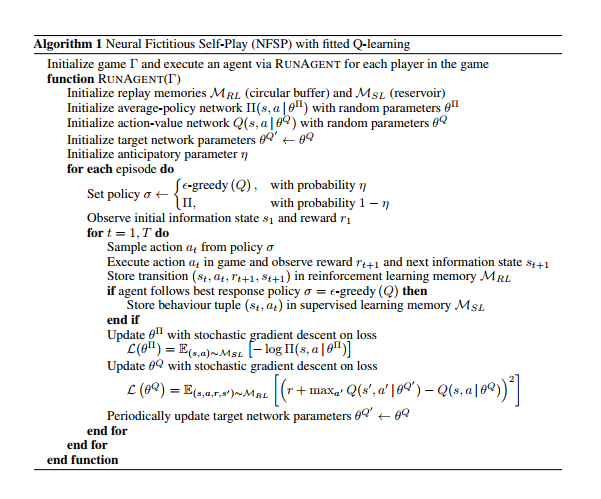
\includegraphics[scale=.8]{images/NFSP_algorithm.png}
    \caption{Neural Fictitious Self-Play\citep{heinrich2016deep}}
\end{figure}

As shown in figure 2.5 at each iteration the policy is selected first.
Next an action $a_t$ is sampled from that policy and by taking that action we generate a reward
and subsequent state.
This information is stored in $M_{RL}$ and conditionally in $M_{SL}$ based on the policy selected.
After this stochastic gradient descent is used to update $\theta^\Pi$ and $\theta^Q$ who's new values
are periodically applied to our neural networks.
Over time the action value and average-policy networks will improve their
accuracy as each player gains experience and learns.
This culminates in an approximate Nash equilibrium as players develop better and better strategies.


\subsubsection{Convergence and Empirical Results}
This algorithm was applied to both Leduc Hold'em and Limit Texas Hold'em with variation in a number
of parameters such as number of hidden layers and neurons in the neural networks.

The best results achieved for Leduc Hold'em used a single hidden layer neural network with 128 hidden neurons.
This instantiation of the algorithm developed a strategy reached exploitability levels of less that .1, with
a starting value of 1.5.

The Limit Texas Hold'em instantiation of the algorithm was tested against the top 3 competitors of
the 2014 ACPC using win rate as the evaluation metric in milli big-blinds per hand (mbb/h).
This saw a trained win rate of between -13 and -52mbb/h against these agents with the initial win rate being
roughly -700mbb/h.